\frame{
\begin{tikzpicture}[remember picture,overlay]
\fill[blue1]
(current page.north west) rectangle ([xshift=12.cm,yshift=-10.cm]current page.east|-{pic cs:end});
\end{tikzpicture}
\textcolor{white}{\Huge
Backup slides}
}

\frame{
	\frametitle{Synthetic radiograms}
	
	\begin{textblock}{0.9}(0.03,0.05)
		\centering
		\includegraphics[width=0.6\textwidth]{Sources/X-DFA/particle_mask_construction.pdf}
	\end{textblock}
	
	\begin{textblock}{0.9}(0.05,0.8)
		\centering
		Beer-Lambert\\
		$I(z_l) = I_0 \exp(-\mu z)$
	\end{textblock}
	
	\begin{textblock}{0.2}(0.03,0.6)
		\visible<2->{
			\includegraphics[width=\textwidth]{Sources/X-DFA/thicknessMap_nPart10.png}}
	\end{textblock}
	
	\begin{textblock}{0.2}(0.77,0.6)
		\visible<2->{
			\frame{
				\includegraphics[width=\textwidth]{Sources/X-DFA/fake_img_nPart10.png}
		}}
	\end{textblock}
}

\frame{
	\frametitle{Linear space invariant imaging}
	\begin{textblock}{0.5}(0.0,0.15)
		\visible<1->{
			\centering
			Image correlation function
			\[
			g(\mathbf{q}, \tau) = \frac
			{\langle I^*(\mathbf{q},t) I(\mathbf{q},t+\tau) \rangle_t}
			{\langle |I(\mathbf{q},t)|^2 \rangle_t}
			\]
		}
	\end{textblock}
	
	
	
	\begin{textblock}{0.5}(0.5,0.15)
		\visible<2->{
			\centering
			Intermediate scattering function
			\[
			f(\mathbf{q},\tau) = \frac
			{\langle \rho^*(\mathbf{q},t) \rho(\mathbf{q},t+\tau) \rangle_t}
			{\langle |\rho(\mathbf{q},t)|^2 \rangle_t}
			\]}
	\end{textblock}
	
	\begin{textblock}{0.9}(0.05,0.42)
		\visible<2->{	
			Linear space-invariant imaging:
			\begin{align}
			I(\mathbf{r},t) = I_0 + \int \mathsf{d}\mathbf{r}' \ \mathsf{d}z'
			T(\mathbf{r}-\mathbf{r}',-z') c(\mathbf{r}',z',t)
			\nonumber
			\end{align}
		}
	\end{textblock}
	
	
	\begin{textblock}{0.9}(0.05,0.6)
		\visible<2->{
			\centering
			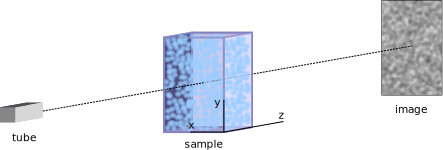
\includegraphics[width=0.7\textwidth]
			{Sources/X-DFA/image_transfer_function1.pdf}
		}
	\end{textblock}	
}

%%%%%%%%%%%%5 Tracking of particle front
\frame{
	\frametitle{Tracking of particle front}
	
	\begin{textblock}{0.9}(0.05,0.1)	
		\centering
		\only<1>{
			\includegraphics[width=0.8\textwidth]
			{Sources/sedimenting_bed/steepest_gradient_gv_profile.pdf}}
	\end{textblock}
}

\frame{
	\frametitle{Tracking of particle front}
	\begin{textblock}{0.7}(0.15,0.1)	
		\centering
		\only<1>{
			\includegraphics[width=\textwidth]
			{Sources/sedimenting_bed/setup-sketch-distortion.pdf}}
	\end{textblock}
	
	
	\begin{textblock}{0.9}(0.05,0.5)
		\only<1>{
			\vspace{-0.5cm}
			\centering
			\includegraphics[width=0.8\textwidth]
			{Sources/sedimenting_bed/image_transfer_function3_track_front_midplane.pdf}}
	\end{textblock}
}

\frame{
	\frametitle{Tracking of particle front}
	\begin{textblock}{0.9}(0.05,0.1)	
		\centering
		\only<1>{
			\includegraphics[width=0.5\textwidth]
			{Sources/sedimenting_bed/steepest_gradient_gv_profile.pdf}}
	\end{textblock}
	
	\begin{textblock}{0.35}(0.02,0.5)	
		\centering
		\visible<1->{
			\includegraphics[width=\textwidth]
			{Sources/sedimenting_bed/plot_extract_edge_pos_mid_plane.png}}
	\end{textblock}
	
	
	\begin{textblock}{0.35}(0.52,0.5)	
		\centering
		\visible<1->{
			\includegraphics[width=\textwidth]
			{Sources/sedimenting_bed/lin_fit_y-pos_vs_time.png}}
	\end{textblock}
}


